\documentclass{standalone}
\usepackage{tikz}
\usetikzlibrary{shadows}
\newcommand{\profile}[1][]{
    \pgfmathsetseed{1234}
    \draw[snowflake,#1] (0:rnd/5) 
        \foreach \i in {1,...,10}{
            -- (rnd*15:rnd*3+\i)
        }
        -- ++(0:1) -- (0:15)
        \foreach \i in {15,...,20}{
            -- (rnd*15:rnd*7+\i)
        }
        -- ++(0:3)
        \foreach \i in {1,3,...,30}{
            -- (\i-rnd*3:30-rnd*3)
        }
        \foreach \i in {20,...,1}{
            -- (30-rnd*10:rnd*3+\i)
        };
}

\begin{document}
    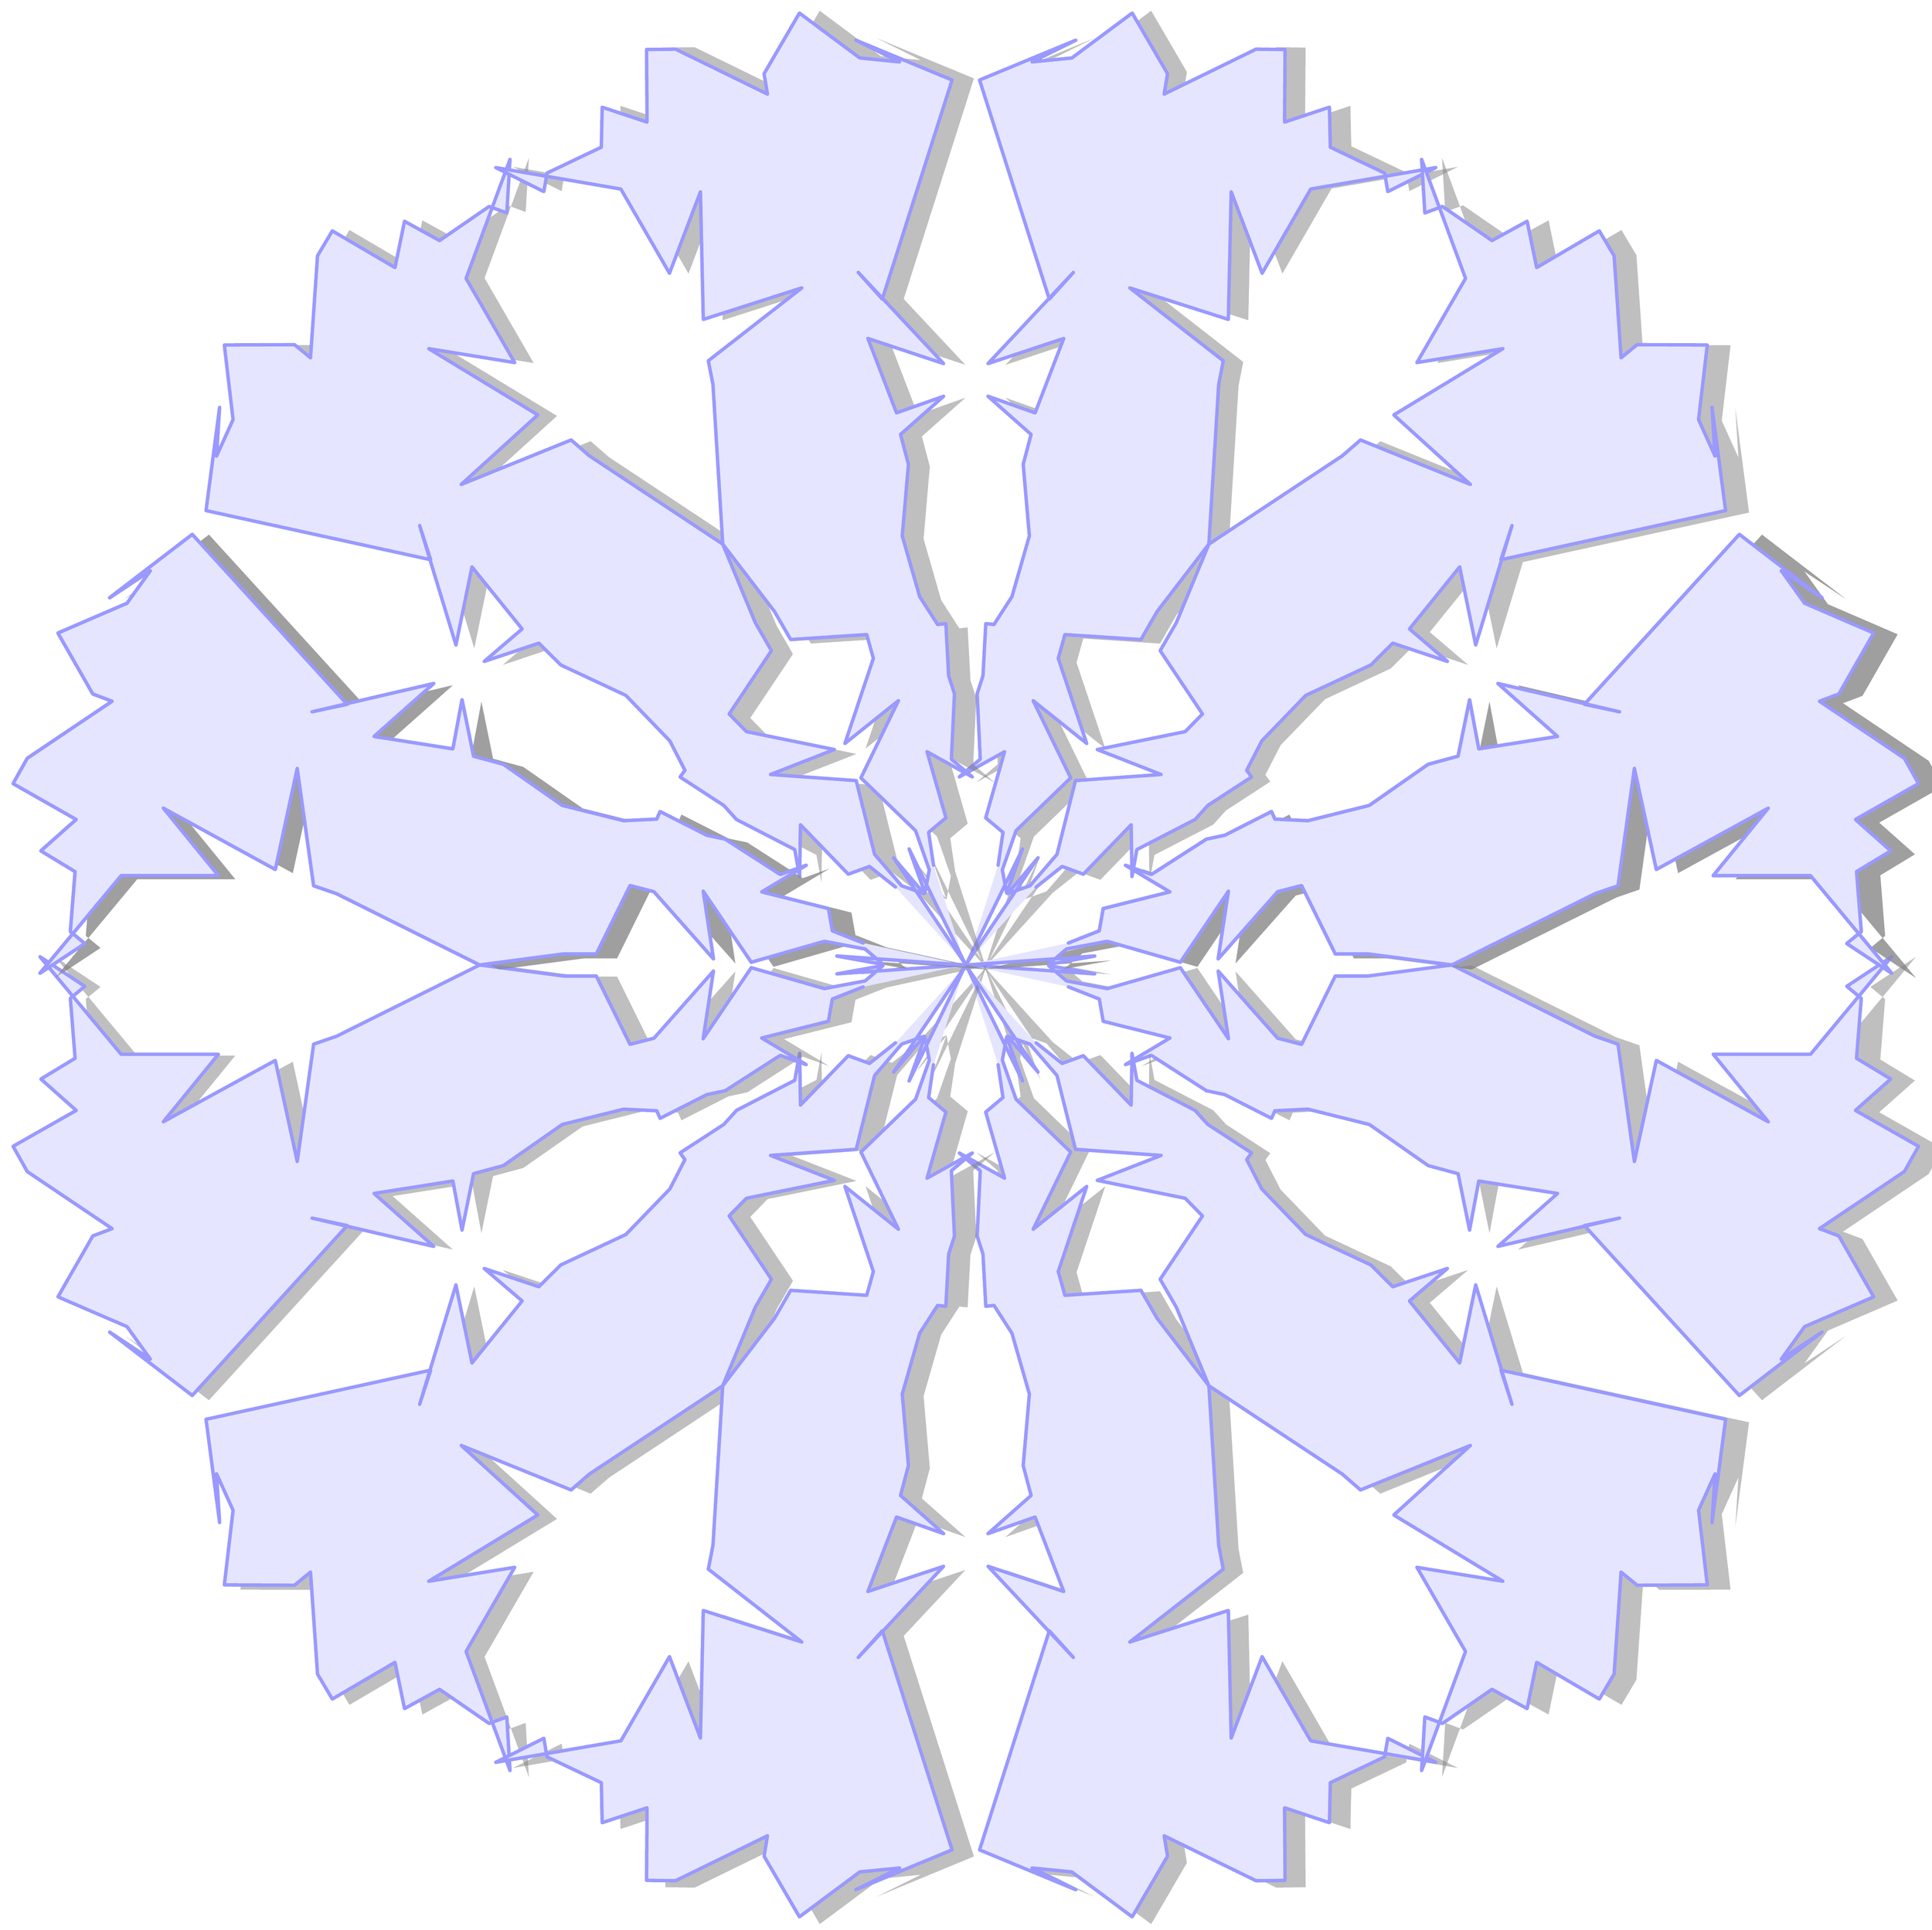
\begin{tikzpicture}[
        snowflake/.style={
            fill=blue!10,
            draw=blue!40,
            drop shadow={shadow scale=1.01,shadow xshift=.6},
            line join=round,
            line cap=round,
            line width=3pt,
        }
    ]
    \foreach \a in {0,60,...,360}{
        \begin{scope}[rotate=\a]
            \profile
            \profile[cm={-1,0,0,1,(0,0)}]
        \end{scope}
    }
    \end{tikzpicture}
\end{document}
